\documentclass{article}

\def\titre{Session 2: Fondamentaux informatique pour bien démarrer les cours et tests de positionnements AP1/APP1}

\usepackage[a4paper,left=20mm,right=20mm,top=25mm,bottom=40mm]{geometry}
\usepackage{enumitem}
\setlist{partopsep=0pt,topsep=1ex}
\usepackage{pifont,euscript}
\usepackage{rotating}
\usepackage{tabu}
\usepackage[usenames,dvipsnames,svgnames]{xcolor}
\usepackage{comment}
\usepackage{colortbl}
\usepackage{titling}
\usepackage{multicol}
\usepackage[french]{babel}
\usepackage{mdframed}
\usepackage{textcomp}
\usepackage{listings}
\lstloadlanguages{Python}

\setlength{\droptitle}{-1.5cm}
\pretitle{\begin{center}\LARGE\sffamily\bfseries}
\posttitle{\par\end{center}\vskip -.5cm}
\preauthor{}
\postauthor{}
\predate{}
\postdate{}

\definecolor{UGEBlue}{RGB}{47,42,133}
\definecolor{vert}{RGB}{78,100,26}
\definecolor{violet}{RGB}{130,25,111}
\definecolor{orange}{RGB}{234,91,12}
\definecolor{rouge}{RGB}{230,56,18}
\definecolor{beige}{RGB}{242,238,231}
\definecolor{bleu}{RGB}{0,74,155}
\definecolor{gris}{RGB}{100,100,100}
\definecolor{commentColor}{rgb}{0.38,0.63,0.69}
\definecolor{stringColor}{rgb}{0.25,0.44,0.63}
\definecolor{typeColor}{rgb}{0.56,0.13,0.00}
\definecolor{keywordColor}{rgb}{0.00,0.44,0.13}
\definecolor{digitColor}{rgb}{0.25,0.63,0.44}

\lstset{ %
  backgroundcolor=\color{white},
  basicstyle=\ttfamily,
  breaklines=true,
  captionpos=b,
  commentstyle={\bfseries\itshape\color{commentColor}},
  escapeinside={\%*}{*)},
  keywordstyle=\color{keywordColor},
  stringstyle=\color{stringColor},
  numbers=left,
  stepnumber=1,
  numberstyle=\scriptsize,
  numbersep=10pt,
  language=Python,
  upquote=true
}
\lstset{%
  literate=%
    {é}{{\'e}}1
    {è}{{\`e}}1
    {ê}{{\^e}}1
    {ë}{{\"e}}1
    {à}{{\`a}}1
    {â}{{\^a}}1
    {ä}{{\"a}}1
    {î}{{\^i}}1
    {ï}{{\"i}}1
    {ù}{{\`u}}1
    {û}{{\^u}}1
    {ü}{{\"u}}1
    {ô}{{\^o}}1
    {ö}{{\"o}}1
    {ç}{{\c c}}1
    {œ}{{\oe{}}}1
    {0}{{{{\color{digitColor}0}}}}1
    {1}{{{{\color{digitColor}1}}}}1
    {2}{{{{\color{digitColor}2}}}}1
    {3}{{{{\color{digitColor}3}}}}1
    {4}{{{{\color{digitColor}4}}}}1
    {5}{{{{\color{digitColor}5}}}}1
    {6}{{{{\color{digitColor}6}}}}1
    {7}{{{{\color{digitColor}7}}}}1
    {8}{{{{\color{digitColor}8}}}}1
    {9}{{{{\color{digitColor}9}}}}1
    {.0}{{{{\color{digitColor}.0}}}}2
    {.1}{{{{\color{digitColor}.1}}}}2
    {.2}{{{{\color{digitColor}.2}}}}2
    {.3}{{{{\color{digitColor}.3}}}}2
    {.4}{{{{\color{digitColor}.4}}}}2
    {.5}{{{{\color{digitColor}.5}}}}2
    {.6}{{{{\color{digitColor}.6}}}}2
    {.7}{{{{\color{digitColor}.7}}}}2
    {.8}{{{{\color{digitColor}.8}}}}2
    {.9}{{{{\color{digitColor}.9}}}}2
    {'h}{{{{\color{digitColor}'h}}}}2
}
\lstset{%
  emph={int,char,void,float,double},
  emphstyle=\color{typeColor}
}

\usepackage{lmodern}
\usepackage{amssymb,amsmath}
\usepackage{ifxetex,ifluatex}
\usepackage[T1]{fontenc}
\usepackage[utf8]{inputenc}
\usepackage{upquote}

\usepackage[unicode=true]{hyperref}
\hypersetup{breaklinks=true,
%            bookmarks=true,
            pdfauthor={},
            pdftitle={\titre},
            colorlinks=true,
            citecolor=blue,
            urlcolor=blue,
            linkcolor=magenta,
            pdfborder={0 0 0}}
\urlstyle{same}  % don't use monospace font for urls
\usepackage{tikz}
\usetikzlibrary{quotes}
\usetikzlibrary{arrows,positioning} 

\tikzstyle{val}=[rectangle,draw]
\tikzstyle{var}=[rectangle,rounded corners=1.5ex,draw,bleu,minimum size=3ex]
\tikzstyle{aff}=[->,thick]
\tikzset{
  every node/.style={font=\footnotesize},
  instr/.style={rectangle,draw=black!70},
  test/.style={rectangle,rounded corners,draw=bleu!70,text=bleu},
  every edge/.style={>=stealth,semithick,bend angle=45,draw,->},
  every edge quotes/.style={inner sep=.5em,font=\scriptsize,color=orange},
  vrai/.style={left,"vrai"},
  faux/.style={right,"faux"},
}
\usepackage{color}
\usepackage{fancyvrb}
\setlength{\parindent}{0pt}
\setlength{\parskip}{6pt plus 2pt minus 1pt}
\setlength{\emergencystretch}{3em}  % prevent overfull lines
\providecommand{\tightlist}{%
  \setlength{\itemsep}{0pt}\setlength{\parskip}{0pt}}
\setcounter{secnumdepth}{5}

\usepackage{fancyhdr}
\fancyhead[L]{
\includegraphics[height=1.1cm]{UPEM-IGM-V1_300dpi.png}}
\fancyhead[C]{{
\bf Pré-rentrée informatique\\
Semaine d'intégration du 5 au 9 septembre 2022\\
}
L1 Informatique \& Mathématiques
}
%\fancyhead[R]{
\includegraphics[height=1.3cm]{logo-ligm.png}}
\setlength{\headheight}{50pt}
\renewcommand{\headrulewidth}{1pt}


% cadres informatifs
\newcommand{\but}[1]{%
\hbox{}\noindent%
\fcolorbox{CadetBlue}{white}{%
  \parbox{\dimexpr\linewidth-2\fboxsep-1pt\relax}{%
    \vskip10pt%
    \leftskip10pt\rightskip10pt%
    #1%
    \vskip10pt}}\medskip\thispagestyle{fancy}}


% Environnements d'exercices

\font\manual=manfnt % font used for the METAFONT logo, etc.
\def\barble{{\manual\char1}}
\def\fulltriangleright{{\manual\char120}} %
\def\fulltriangleup{{\manual\char54}} %
\def\fulltriangledown{{\manual\char55}}
\def\littlecube{{\manual\char28}}
\def\prettystar{{\manual\char30}}
\def\littlecircles{{\manual\char36}}
\def\littlelosanges{{\manual\char37}}
\def\littlecloud{{\manual\char38}}
\def\ellipsoid{{\manual\char88}}
\def\zip{{\manual\char121}} % -/\/->
\def\dbendright{{\manual\char126}}
\def\dbendleft{{\manual\char127}}
\def\question{\noindent\llap{\ding{90}\ding{212}}{\kern1pc}}
\newcounter{exo_count}
\def\exoname{Exercice}
\newenvironment{exercice}[1][]%
{\smallbreak\refstepcounter{exo_count}%
\vspace{0.3cm}%
\begin{sloppypar}\noindent{\fulltriangleright\kern 2pt%
\bf\exoname~\arabic{exo_count} : #1} %
}%
{\end{sloppypar}%
}



\newenvironment{correction}{\subsection*{\textcolor{red}{Correction}}}{\medskip}

\def\labelenumi{\arabic{enumi}.}
\def\labelenumii{\alph{enumii}.}

\title{\color{UGEBlue}\titre}
%\date{Semestre 2}
\date{}


\newcommand{\code}[1]{\lstinline{#1}}
\lstnewenvironment{fullcode}{\lstset{xleftmargin=1.4em}}{}
\lstnewenvironment{nonumbercode}{\lstset{numbers=none}}{}


\excludecomment{correction}
% Commenter la ligne ci-dessus si on souhaite afficher les corrections

\begin{document}
\maketitle

\but{Dans ce TP vous allez:
\begin{itemize}
\item Être initié à la pratique du terminal Unix : interface Shell, système de fichiers, redirection, archivage et droits;
\item Utiliser le terminal pour exécuter un notebook Jupyter et un programme Python;
\item Manipuler l'IDE Thonny ainsi que PythonTutor qui seront utilisés pour les cours de Python (AP1/APP1);
\item Présentation de l'exerciseur PLaTon.
 \end{itemize} 
}

\section {Pratique du terminal et de l’arborescence des fichiers Unix}

Dans cette section, nous allons parler du Terminal, un outil puissant et incontournable sous unix! Dans les exercices suivants, votre souris fait la sieste, vous ne devez surtout pas la réveiller !
Essayez de jouer le jeu SVP.

L'interaction avec un système d’exploitation (OS) peut se faire sous deux formes : soit une interface graphique utilisateur avec une souris et tout (Session 1), soit une interface en ligne de commande uniquement avec le clavier (Session 2) : il s'agit du Terminal. 

Il est parfois plus efficace d’interagir avec le système via le clavier. Le terminal vous met en communication avec un interpréteur de
commandes UNIX : le shell (notez cependant que la plupart des gens utilisent le terme ``shell'' pour désigner l’interface en ligne de commande uniquement).

Il existe plusieurs types de Shell, sous Linux, le nôtre s’appelle bash. Il en existe d’autres comme sh, csh, tcsh, ksh, zsh.
Le shell vous permet de lancer des commandes, de les enchaîner, et surtout d’automatiser l’exécution d’un certain nombre de tâches.

Une interface en ligne de commande est beaucoup plus austère et peut paraître primitive par rapport à une interface graphique. Celle-ci se présente sous la forme d’une grande boîte noire dans laquelle l’utilisateur va taper des commandes (généralement une commande par ligne) pour interagir avec son OS.

Dans une interface en ligne de commande, il n’y a aucun usage de la souris : tout se fait via l’entrée de commandes tapées au clavier. Les interfaces en ligne de commande peuvent être en fait très puissantes et permettre de réaliser des opérations complexes beaucoup plus rapidement qu’avec une interface graphique.

Les shells exigent donc que l’utilisateur connaisse certaines commandes et leur syntaxe et comprenne les concepts relatifs au langage de script spécifique au shell utilisé.

Dans la suite de cette rapide initiation, nous verrons quelques commandes de bases pour le shell Linux. 

\begin{exercice}[Premier pas avec le terminal]

\begin{enumerate}
\def\labelenumi{\arabic{enumi}.}
\item
  En utilisant le menu des applications, ouvrez un terminal. Le terminal
  vous indique qu'il est prêt en affichant une invite (ou
  \emph{prompt}), en général le caractère dollar \texttt{\$} ou
  supérieur \texttt{\textgreater{}}, en début de ligne.  
\item
Le terminal s'ouvre automatiquement dans votre répertoire personnel, pour le vérifier taper la commande \texttt{pwd}. 
Vous devriez avoir le retour suivant \texttt{/home/login} (ou ``login'' est votre login)
\texttt{pwd} est une commande très importante qui vous permet de toujours savoir où vous êtes. Cette commande vous indique votre répertoire de travail (ou répertoire courant). 
Le résultat est toujours un chemin absolu.
\item
  Essayez les commandes \texttt{echo\ bonjour}, puis
  \texttt{echo\ -n\ bonjour}. Ici, \texttt{echo} est le nom de la
  commande, \texttt{bonjour} est un \emph{argument}, et \texttt{-n} est
  une \emph{option}. Pouvez-vous deviner à quoi sert la commande
  \texttt{echo} ? Et l'option \texttt{-n}?
\item
  La commande \texttt{man} sert à consulter la documentation de
  n'importe quelle commande du système. Pour l'utiliser, on tape
  \texttt{man} suivi du nom de la commande souhaitée. Utilisez cette
  commande pour consulter la documentation de la commande \texttt{echo}.
\item
  Testez la commande \texttt{ls} et regarder la page du manuel
  correspondant à cette commande pour expliquer quelle est sa fonction et ses différentes options.
\item
  À l'aide de cette commande et des options vues dans le manuel, déterminez à quel moment le répertoire
  ``preRentree''  (créée en session 1) a été modifié pour la dernière fois.

\begin{correction}
  \textcolor{red}{il faut utiliser \texttt{ls -l}}
\end{correction}

\end{enumerate}
\end{exercice}

\subsection{Quelques astuces pour aller plus vite}

\begin{enumerate}
\item
  Vous pouvez utiliser les flèches ``haut'' et ``bas'' pour faire
  défiler l'\emph{historique des commandes} que vous avez déjà tapées.

\item
  Vous pouvez utiliser la touche ``tab'' pour compléter un nom de
  commande ou un nom de fichier.
  
\item
  Pour interrompre une commande on peut utiliser la combinaison \texttt{ctrl+c}.
  
\item
  Pour lier les commandes, on sépare les commandes par le caractère `` ; ''
  exemple \texttt{who ; date}

\item
 Pour se déconnecter, il suffit de taper \texttt{exit} ou la combinaison de touches \texttt{ctrl+d}.

\end{enumerate}

\subsection{La commande man et quelques commandes utiles}

Vous l'avez vu lors de l'exercice précédent, une des premières commandes à connaître est la commande \texttt{man}.
Comme vous avez pu le constater, elle affiche dans le terminal le manuel de la commande que vous placez en argument.
Elle permet bien plus et nous allons le voir dans la suite.

\begin{exercice}[Comprendre la commande \texttt{man}]

\begin{enumerate}
\def\labelenumi{\arabic{enumi}.}
\item
  La documentation de \texttt{man} est très complète\ldots{} Faites afficher un résumé
  de ce que vous pouvez faire avec la commande \texttt{man}.\\
  \textbf{Indication: }\texttt{man} est une commande comme les autres et ... comment affiche-t-on l'aide d'une commande ?
\item
  Utilisez la commande \texttt{touch} avec \texttt{preRentree} comme argument.
\item
  À quoi sert la commande \texttt{touch}? Si vous ne voyez pas, pensez à
  utiliser \texttt{ls}
\begin{correction}
  \textcolor{red}{La commande touch \texttt{touch preRentree} va en fait changer la date de création du répertoire preRentree}
\end{correction}

\item
  Que se passe-t-il si vous tapez \texttt{touch\ un\_autre\_fichier.txt}?
\item
  Vous voulez maintenant trouver comment \emph{effacer} un fichier mais
  vous ne savez pas comment s'appelle la commande. \\
  Utilisez \texttt{man\ -k} pour la trouver. Attention cette commande permet de chercher
  une suite de caractères donc la cass, les accents et l'orthographe
  sont importants.
  Vous pouvez par exemple chercher  avec \texttt{man -k file} puis penser à comment dire effacer en anglais \\
  \textbf{À noter : }\texttt{apropos} est aussi une commande qui peut remplacer \texttt{man -k}

\begin{correction}
\textcolor{red}{\c ca va les faire chercher pas mal mais la vraie commande est rm.
En plus se sera avec l'option -i et il faudra répondre par yes}
\end{correction}

\item
  Effacez le fichier \texttt{un\_autre\_fichier.txt}.

  \textbf{Attention !} L'effacement en utilisant la commande du terminal
  est \emph{définitif}. Vous ne retrouverez pas votre fichier dans la
  corbeille ensuite\ldots{}
\item
  Comment faire pour que cette commande vous demande confirmation avant
  de détruire un fichier?
\begin{correction}
\textcolor{red}{ se sera avec l'option -i et il faudra répondre par yes}
\end{correction}
\end{enumerate}

\end{exercice}

\newpage

\begin{exercice}[Quelques commandes très utiles pour la suite]

\begin{enumerate}
\def\labelenumi{\arabic{enumi}.}
\item
  Regardez ensuite les pages du manuel de \texttt{cp}, \texttt{mkdir},
  \texttt{rmdir}, \texttt{rm} et \texttt{cat}.
  Notez qu'il est possible que certaines de ces pages soient en anglais. Rappelez-vous bien des actions de ces commandes.
\item
  La commande \texttt{cd} (pour Change Directory) est aussi une commande très importante. C'est grâce à elle que vous pourrez vous déplacer dans l'arborescence de fichiers. 
  Elle n'a cependant pas de page de manuel dédiée car sa description se trouve dans la page de manuel de \texttt{bash}. 
  Ouvrez la page de manuel de \texttt{bash} (avec \texttt{man bash}) et cherchez la description de la commande \texttt{cd} en
  utilisant la fonctionnalité de recherche suivante: tapez \texttt{/cd}
  pour chercher le mot ``cd'' dans la page puis utiliser la touche
  \texttt{n} pour trouver l'occurence suivante et \texttt{N} pour
  trouver l'occurence précédente. (Si vous ne connaissez pas le mot occurence, cherchez sa définition sur internet.)
\item
 En utilisant la commande \texttt{cd (suivi de quelque chose)}, déplacez vous dans le répertoire ``preRentree'' créé précédemment.
\item
 Utiliser à nouveau la commande \texttt{pwd} pour vérifier que vous avez bien changé de répertoire de travail.
\item
 Avec la commande \texttt{ls} faites apparaître le contenu de ce répertoire. Normalement vous y trouverez deux fichiers créés en session 1.
\item
Avec la commande \texttt{cat}, affichez le contenu des deux fichiers du répertoire (en une seule ligne SVP).

\begin{correction}
\textcolor{red}{il faut utiliser la commande \texttt{cat presentationNomPrenom.txt contacts.txt}}
\end{correction}

\item
À présent comment faire pour remonter à la racine de votre répertoire personnel ? Essayez la commande \texttt{cd ..}
\end{enumerate}

\end{exercice}

\hypertarget{manipuler-larborescence-des-fichiers-dans-le-terminal}{
\subsection{Manipuler l'arborescence des fichiers dans le
terminal}\label{manipuler-larborescence-des-fichiers-dans-le-terminal}}

Vous allez créer une arborescence de fichiers que vous utiliserez dans les exercices suivants. Quand vous ne savez pas quelle commande appeler, pensez à utiliser \texttt{man\ -k} et surtout à regarder l'exercice précédent.

Étant donné que le but de l'exercice est d'apprendre à se servir du terminal pour
manipuler une arborescence de répertoire, continuez à laisser votre souris tranquille !

\begin{exercice}[Création et manipulation de répertoire]

\begin{enumerate}
\def\labelenumi{\arabic{enumi}.}
\item 
Vérifiez que vous êtes bien dans votre répertoire personnel
\item
  À l'aide du terminal, créez-y deux sous-répertoires \texttt{Session\_1} et \texttt{Session\_2}.
\item
  En utilisant la commande \texttt{mv}, déplacez les fichiers 
  \texttt{``presentationNomPrenom.txt''} et \texttt{``contacts.txt ''} créés au TP précédent dans le répertoire \texttt{Session\_1}.
\item
  Vérifiez que vous avez bien déplacé les fichiers comme il le fallait
\item
  Placez-vous à présent dans le sous-répertoire \texttt{Session\_2} et créez le fichier \texttt{cours\_{Session\_2}.txt} que nous utiliserons dans un autre exercice. 
\item
Remontez d'un cran dans la hiérarchie des fichiers et créez un nouveau sous-répertoire \texttt{Repertoire\_{A\_{Supprimer}}}
\item 
Dans ce répertoire, créez le fichier \texttt{fichier\_exemple.txt} puis remontez d'un cran dans la hiérarchie.
\item
Et maintenant .... supprimer ce répertoire ! Le pouvez-vous ? Pourquoi ? 

\begin{correction}
\textcolor{red}{On ne le peut pas parce que le répertoire n'est pas vide}
\end{correction}

\end{enumerate}

\end{exercice}

\begin{exercice}[Un point sur la notion de chemin relatif VS absolu]

Un chemin est la façon dont vous vous référez aux fichiers et aux répertoires. Il fournit l'emplacement d'un fichier ou d'un répertoire dans la structure de répertoires Linux. 
Un chemin se compose d'un nom et d'une syntaxe de barre oblique : \texttt{/home/login} par exemple (ou login est votre nom de login).

En tant qu'utilisateur, vous devrez utiliser un chemin lorsque vous souhaitez accéder à un certain fichier ou répertoire ou lorsque vous devez donner l'emplacement
d'un fichier ou d'un répertoire à une commande ou à un script.

\subsubsection*{Comprendre la différence entre les chemins absolus et relatifs}\label{Comprendre la différence entre les chemins absolus et relatifs}

La structure des répertoires sous Linux ressemble à la racine d'un arbre. Tout commence à la racine et se ramifie à partir de là.

Si le chemin commence par une barre oblique "/", cette première barre indique la racine (c'est-à-dire root). Le reste des barres obliques dans le chemin ne sont que des séparateurs. 

Le chemin absolu commence toujours à partir du répertoire racine (/). Par exemple, \texttt{/home/login/preRentree/Session\_1}

\begin{enumerate}

\item 
Un chemin relatif commence à partir du répertoire courant (le répertoire de travail). Par exemple, si vous vous trouvez dans le répertoire \texttt{/preRentree} et souhaitez afficher les informations du fichier \texttt{``contacts.txt''} du répertoire \texttt{Session\_1} vous pouvez utiliser \texttt{ ls -l Session\_1/contacts.txt}. Il s'agit du chemin relatif (à partir du répertoire courant, sans ``/''). Pour mieux comprendre regardez les commentaires marqués d'un (1) sur le schéma de la figure 1.

\medskip

\item
Si vous êtes dans le répertoire \texttt{Session\_1/} et que vous voulez accéder directement au répertoire \texttt{Session\_2/}, vous pourriez utiliser \texttt{cd /home/login/preRentree/Session\_2}, soit le chemin absolu. Pour mieux comprendre regardez les commentaires marqués d'un (2) sur le schéma de la figure 1.

\end{enumerate}

Faites-vous même les tests pour vérifier que vous avez bien compris.

\begin{figure}[h!]
    \begin{center}
    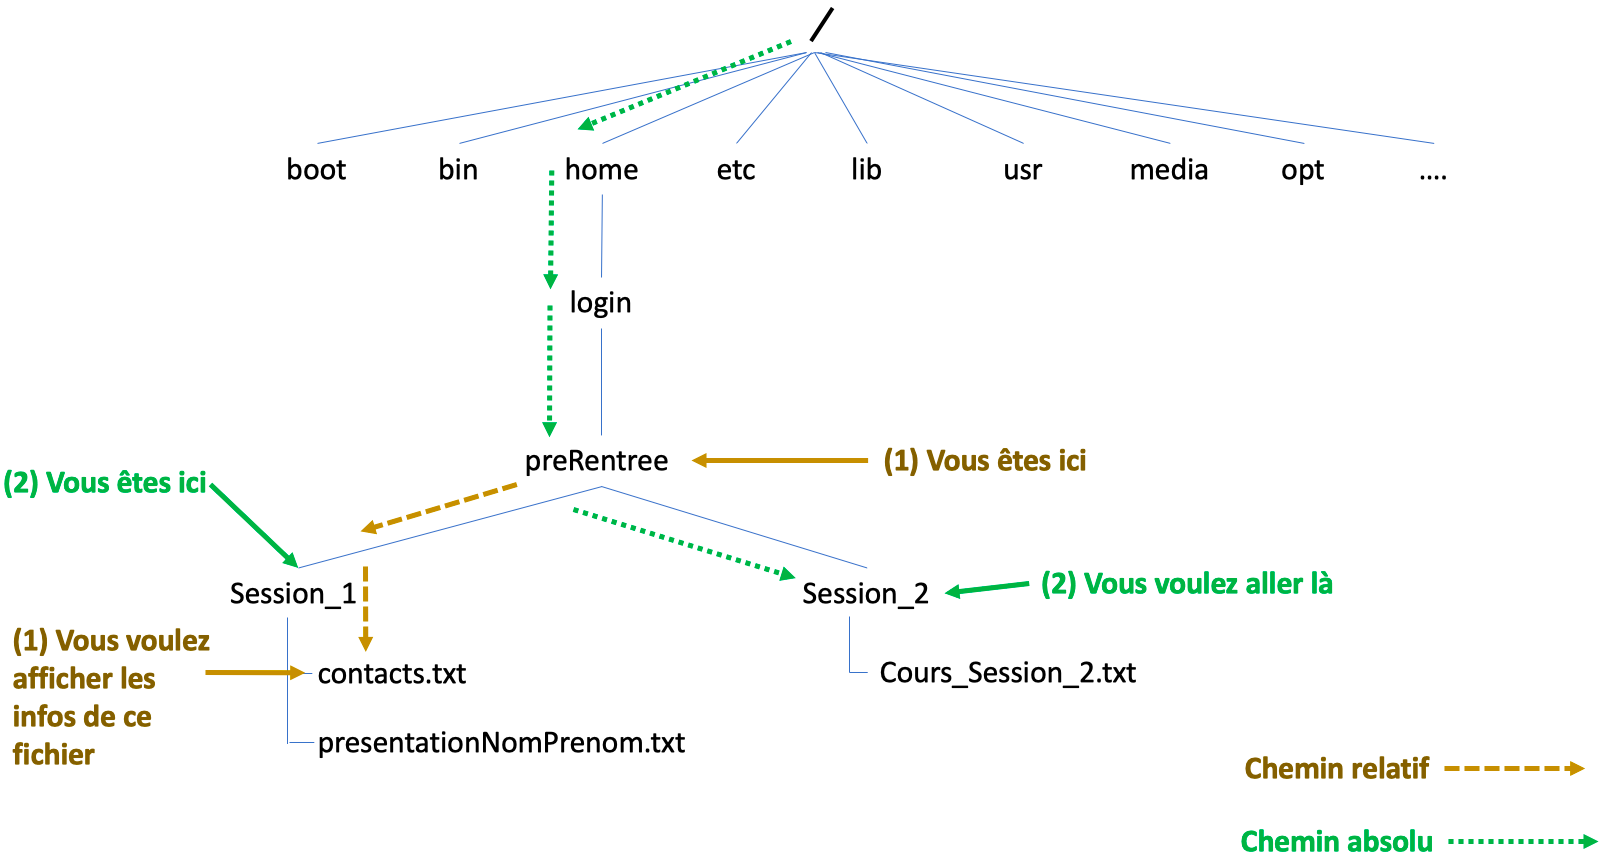
\includegraphics[scale=0.3]{chemin_1.png}
    \caption{Schéma simplifié de l'arborescence de vos fichiers}
     \end{center}
\end{figure}    

\subsubsection*{Utiliser les chemins relatif spéciaux avec . et .. répertoires}\label{Utiliser un chemin relatif avec . et .. répertoires}

Il existe d'autres moyens pour utiliser le chemin relatif :  

    . (un seul point) indique le répertoire courant dans le chemin.    
        
    .. (deux-points) indique le répertoire parent, c'est-à-dire un niveau au-dessus.

\begin{enumerate}

\item
Vérifiez dans quel répertoire courant vous vous trouvez avec la commande \texttt{pwd}, puis tapez la commande  \texttt{cd .}. Tapez à nouveau \texttt{pwd}, que se passe-t-il ? 

Il peut sembler étrange d'avoir une commande spéciale représentant un état sans changement, mais c'est une directive utilement explicite. Imaginez par exemple, que dans les répertoires \texttt{Session\_1} et \texttt{Session\_2} il y ait un fichier exécutable portant le même nom. Imaginons que ce soit des programmes de configurations de votre environnement, avec des configurations radicalement différentes. À chaque fois que vous utiliseriez ces programmes personnalisés, vous voudriez faire attention à ce que votre ordinateur sache exactement quel commande exécuter.

\medskip

\item
Si vous êtes dans le répertoire \texttt{Session\_2} et que vous voulez accédez directement au répertoire \texttt{Session\_1}, au lieu d'utiliser \texttt{cd /home/login/preRentree/Session\_1}, soit le chemin absolu, vous pourriez utiliser la commande  \texttt{cd ../Session\_1}.
Vous l'avez compris les ``..'' vous emmènent directement au répertoire parent qui est \texttt{preRentree}.

\medskip

\item
À présent à partir de votre répertoire courant (normalement \texttt{Session\_1}) utilisez, en une seule fois, le chemin relatif ``..'' pour remonter à la racine ``/''. Pour vous aidez, regardez à nouveau la hiérarchie de la figure 1.

\medskip

\item
Et maintenant place à la découverte, vous avez le droit de vous ``balader'' dans les différents répertoires en dessous de la racine et de vous déplacer de répertoire en répertoire avec les chemins relatifs et/ou absolus. N'oubliez pas non plus de lister le contenu de ces répertoires.
Naturellement ne touchez à rien, ne supprimez pas de fichiers et n'en créez pas d'autre ailleurs que dans votre dossier personnel.

\end{enumerate}

\textbf{Astuce :} la commande \texttt{cd} (seule) permet de retourner à votre répertoire personnel.

\end{exercice}

\hypertarget{Redirections}{
\section{Redirections}\label{Redirections}}

Les redirections sont l'une des plus importantes possibilités offertes par le shell.
Unix utilise des canaux d'entrées/sorties pour lire et écrire ses données. Par défaut le canal d'entrée est le clavier, et le canal de sortie, l'écran. Un troisième canal, le canal d'erreur, est aussi redirigé vers l'écran.
Il est donc possible de rediriger ces canaux vers des fichiers, ou du flux texte de manière transparente pour les commandes Unix.

\begin{exercice}[En sortie]

On se sert du caractère `` > '' pour rediriger la sortie standard (celle qui va normalement sur écran). On indique ensuite le nom du fichier où seront placés les résultats de sortie.

\begin{enumerate}

\item
Revenez dans le répertoire de la \texttt{Session\_2} et rappelez-vous que vous avez créé un fichier \texttt{cours\_{Session\_2}.txt} encore vide. \\
Vous allez le remplir en utilisant la commande suivante : \\
\texttt{echo ``Je suis les cours de la \_Session\_2'' > cours\_Session\_2.txt}
\item
En tapant la commande \texttt{cat cours\_Session\_2.txt} que voyez vous ?
\item
À présent taper la commande \texttt{echo `` Et je suis très heureux !'' > cours\_Session\_2.txt}
\item
En tapant la commande \texttt{cat cours\_Session\_2.txt} que voyez vous ?
\item
Pour éviter cette situation utiliser la double redirection ``\verb+>>+'' (refaites donc toutes les opérations précédentes)

\end{enumerate}

\end{exercice}

\begin{exercice}[En entrée]

Les commandes qui attendent des données ou des paramètres depuis le clavier peuvent aussi en recevoir depuis un fichier, à l'aide du caractère ``< ''. 
Un exemple avec la commande ``wc'' (word count) qui permet de compter le nombre de lignes, de mots et de caractères d'un fichier.

\begin{enumerate}
\item
Testez donc la commande \texttt{wc < cours\_{Session\_2}.txt} et regardez le résultat.
\item
Utilisez la commande \texttt{cat} pour afficher le contenu du fichier \texttt{Session\_2.txt} et comparez ``manuellement'' le résultat précédent.
\item
On peut aussi utiliser à la fois les deux types de redirection : \texttt{wc < cours\_{Session\_2}.txt > compte.txt}.
\end{enumerate}

\textbf{À noter : } Si le fichier résultant n'existe pas la commande \texttt{cat} le créera.

\end{exercice}

\hypertarget{Lancer un serveur jupyter notebook, exécuter un programme python et créer une archive}{
\section{Lancer un serveur jupyter notebook, exécuter un programme python et créer une archive}\label{Lancer un serveur jupyter notebook, exécuter un programme python et créer une archive}}

Ici on passe à une pratique en rapport plus ``direct'' avec les cours que vous allez ``subir'' par la suite :-) en particulier AP1 et APP1. Pour les autres promotions cela ne fera pas de mal de manipuler un peu aussi. 

\begin{exercice}[Décompresser et exécuter un notebook jupyter à partir du terminal]

Vous avez à nouveau le droit d'utiliser votre souris mais juste pour cet exercice ! 
Allez sous Elearning dans la partie réservée à la session 2 et téléchargez le fichier compressé \texttt{preRentree\_Jupyter.zip} que vous placerez dans votre répertoire \texttt{Session\_2}.\\
\textbf{Fin de l'utilisation de la souris et retour au terminal !}

\begin{enumerate}

\item
À partir du terminal décompresser ce fichier avec la commande \texttt{unzip}
\item
Une fois décompressé, vous devriez voir apparaître un nouveau répertoire \texttt{preRentree\_Jupyter}. Déplacez vous à l'intérieur de ce répertoire pour voir apparaître le notebook jupyter \texttt{preRentree\_Jupyter.ipynb}. Il s'agit du notebook source de celui que vous avez vu en \texttt{Session\_1}. 
\item
Il y a deux fa\c cons de procéder pour lancer un notebook jupyter :

\begin{enumerate}
\item
La première méthode vous permettra de voir et de manipuler le serveur de notebook jupyter installé sur les machines des salles de TP. Pour ce faire tapez la commande suivante 
\texttt{jupyter notebook}.\\
Une fois le serveur lancé cliquez sur le notebook \texttt{preRentree\_Jupyter.ipynb}.\\
Si vous vous souvenez de la \texttt{Session\_1}, vous devriez retrouver des similitudes avec l'application MyBinder (voir vidéo ``serveur\_jupyter.mov'').\\
Pour arrêter un serveur jupyter, la meilleure méthode est de retourner sur le terminal et de taper la combinaison \texttt{ctrl+c} puis de valider par ``y'' pour dire ``yes''.
\medskip

\item
La deuxième méthode lance directement le serveur jupyter et le notebook jupyter. Il suffit de taper la commande \texttt{jupyter notebook preRentree\_Jupyter.ipynb}. La suite est exactement la même qu'avec la méthode précédente.
\end{enumerate}

\end{enumerate}

\end{exercice}

\begin{exercice}[Mon premier programme Python]

Parlons encore plus sérieusement ! Ici vous allez écrire et exécuter votre premier programme python.
Pour l'occasion vous allez apprendre à lancer l'éditeur de texte à partir du terminal. 

\begin{enumerate}

\item
Replacez-vous dans le répertoire de la \texttt{Session\_2}
\item
Créer un fichier \texttt{monProgramme.py}
\item
Ouvrez ce fichier dans un éditeur de texte avec la commande \texttt{gedit monProgramme.py}. Via cette commande vous ouvrez l'application ``Éditeur de texte'' de votre Linux Debian.
\item
Écrivez la seule phrase suivante \texttt{print(``Hello World !'')} et enregistrez le fichier (vous avez le droit à la souris).
\item
À présent vous allez exécuter votre premier programme python à l'UGE et voici comment faire : tapez la commande \texttt{python3 monProgramme.py}.\\ 
Si tout c'est bien passé vous devriez voir apparaître dans le terminal la phrase \texttt{Hello World !}.
\end{enumerate}

\textbf{À noter : } la commande utilisée pour exécuter ce script python (on dit bien script) est particulière. Sans rentrer dans les détails il y a deux versions (ou branche) du langage Python : 2 et 3. La version actuellement la plus utilisée est la numéro 3. Il est nécessaire de faire appel à cette commande pour permettre au système de comprendre que l'utilisateur souhaite exécuter un script Python. 

\end{exercice}

\begin{exercice}[Créer une archive]

Il est temps de boucler la boucle ! Puisque vous avez téléchargé une archive compressée au format ZIP à l'exercice 8, vous allez créer une nouvelle archive au format ZIP que vous uploaderez sur le Elearning. 
Toujours à l'aide du terminal, dans cet exercice nous vous demandons : 

\begin{enumerate}
\item 
De vous déplacez dans le répertoire de la \texttt{Session\_2} et de créer un nouveau répertoire \texttt{Nom\_Prenom\_Session\_2} (où Nom et Prenom sont les votres)
\item 
De déplacez les fichiers \texttt{monProgramme.py} et \texttt{cours\_{Session\_2}.txt} dans le répertoire \texttt{Nom\_Prenom\_Session\_2} que vous avez créé précédemment.
\item 
De compresser ce même répertoire à l'aide de la commande \texttt{zip -r Nom\_Prenom\_Session\_2.zip Nom\_Prenom\_Session\_2} (consulter man zip)
\item
Avec la souris cette fois, uploader cette archive sous Elearning dans le répertoire ``Zone de rendu de l'exercice 10''
\end{enumerate}

\textbf{À noter : } il existe plusieurs fa\c cons de compresser et d'archiver sous unix, mais cela nécessiterait plusieurs chapitres et ce n'est pas le but ici. Pour les plus curieux et curieuses il y a la commande \texttt{tar} que vous pourriez aller voir ...

\end{exercice}


\hypertarget{(En fonction du temps) Notions de propriétés et droits d'accès}{
\section{(En fonction du temps) Notions de propriétés et droits d'accès}\label{(En fonction du temps) Notions de propriétés et droits d'accès}}

Dans tout système d'exploitation, en particulier Unix, il est nécessaire de protéger le
fonctionnement du système en interdisant certaines actions à l'utilisateur.\\
Pour cela, il existe une notion de ``droits'' (ou ``permissions'') et de ``groupe''. \\
Chaque fichier et répertoire, possède des droits qui lui sont propre, des autorisations d'accès individuelles. 
Lors d'un accès, le système vérifie si celui-ci est permis selon la catégorie (le groupe) de l'utilisateur.

\hypertarget{droits-des-répertoires-et-des-fichiers}{
\subsection{Droits des répertoires et des fichiers}\label{droits-des-répertoires-et-des-fichiers}}

\begin{exercice}[Affichage des droits]

Pour afficher à l'écran les droits alloués à un répertoire ou un fichier, il faut utiliser la commande \texttt{ls -l} qui permet de lister toutes les 
informations connexes possibles dont les droits des répertoires et des fichiers. 

\begin{enumerate}

\item
Déplacez-vous dans votre répertoire \texttt{preRentree} et tapez la commande \texttt{ls -l} pour voir apparaître les droits sur vos répertoires \texttt{Session\_1} et \texttt{Session\_2}. 
Vous devriez voir apparaître les lignes suivantes.\\
Dans la figure 2 suivante, seules les informations intéressantes ont été affichées.

\begin{figure}[h!]
    \begin{center}
    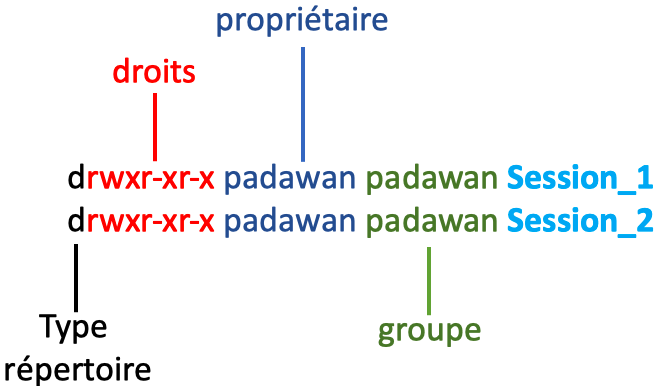
\includegraphics[scale=0.2]{droitsRep.png}
    \caption{Droits sur les répertoires \texttt{Session\_1} et \texttt{Session\_2}}
     \end{center}
\end{figure}    

\medskip

\item
Faites de même sur le répertoire \texttt{Session\_1} pour voir apparaître les droits sur les fichiers \texttt{``presentationNomPrenom.txt''} et \texttt{``contacts.txt ''}.
Dans la figure 3 suivante, seules les informations intéressantes ont été affichées.

\begin{figure}[h!]
    \begin{center}
    
\includegraphics[scale=0.2]{droitsFichier.png}
    \caption{Droits sur les fichiers du répertoire \texttt{Session\_1}}
     \end{center}
\end{figure}    

\end{enumerate}

\newpage

Les droits sont représentés par une suite de 9 caractères. 

\begin{enumerate}
\item
Les trois premiers sont les permissions de l'utilisateur propriétaire du fichier ou du répertoire, seul à même de changer les droits ou le groupe de son fichier et/ou répertoire.
\item
Les trois suivants celles du groupe auquel appartient le propriétaire (cela pourrait être le domaine de l'UGE par exemple). Un groupe d'utilisateurs est un ensemble d'utilisateurs 
privilégiés ayant en général des permissions moindres que le propriétaire d'un fichier mais plus grandes que la catégorie qui suit.
\item
Les trois dernières celles de tous les autres utilisateurs.
\end{enumerate}

\begin{figure}[h!]
    \begin{center}
    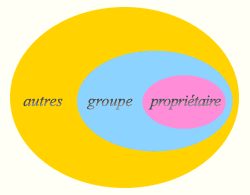
\includegraphics[scale=0.6]{droits2.png}
    \caption{Modèle concentrique des droits d'accès}
     \end{center}
\end{figure}    

Le schéma ci-haut montre qu'un ensemble de propriétaires forme un groupe, qu'un ensemble de groupes forme la catégorie "autres" (qui sont tous ceux qui prétendent à accéder aux données).
L'accès à un sous-ensemble concentrique suppose a priori d'obtenir des droits supplémentaires. 

À chacune des 3 catégories d'utilisateurs, on associe une des 8 combinaisons différentes possibles pour l'allocation des droits que la figure suivante récapitule. 

\begin{figure}[h!]
    \begin{center}
    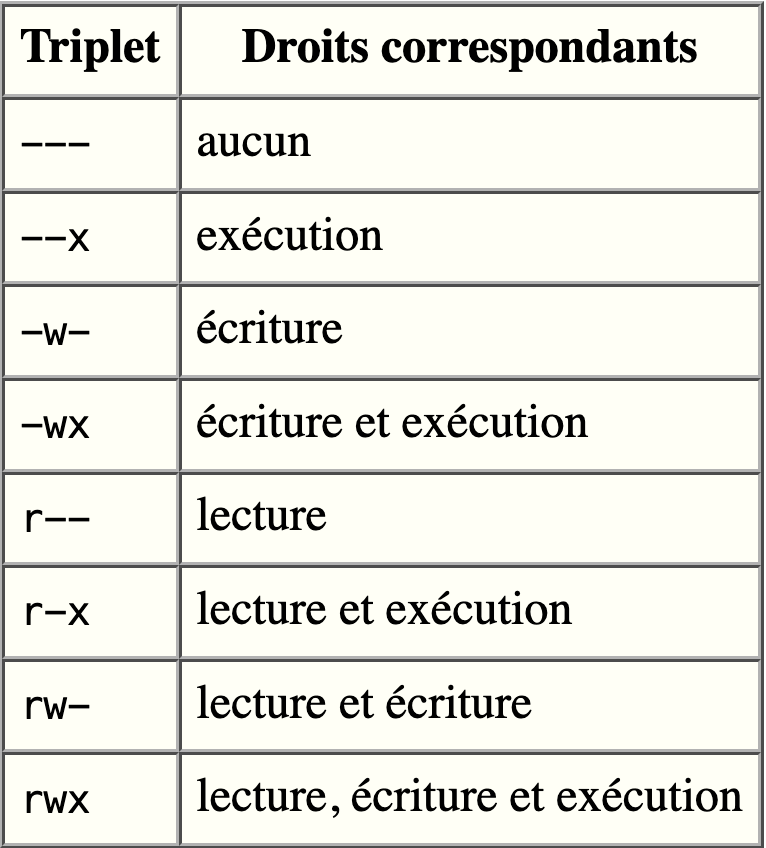
\includegraphics[scale=0.2]{ListeDroits.png}
    \caption{Combinaison des droits}
     \end{center}
\end{figure}    

\newpage

\end{exercice}

\hypertarget{Modifier les droits d'accès}{
\subsection{Modifier les droits d'accès}\label{Modifier les droits d'accès}}

Lors de sa création, un fichier ou un répertoire dispose de droits par défaut. Il est offert au propriétaire d'un fichier (et seulement à lui) de modifier les droits du fichier. C'est-à-dire qu'il peut supprimer des droits ou bien en rajouter de nouveaux à chacune des trois catégories d'utilisateurs. 
Pour cela, on utilise la commande \texttt{chmod} (change mode) selon la syntaxe suivante :  \texttt{chmod} \emph{liste\_droits} \underline{fichier(s)} 

\texttt{chmod} permet d'accorder ou de retirer au(x) fichier(s) et répertoires passé(s) en arguments les permissions
correspondant à \emph{liste\_droits} pour une/des catégorie(s) d'utilisateur(s) cible(s) (propriétaire, groupe ou autre). 

Pour affecter à chaque catégorie la liste des droits voulus, on utilise souvent une notation symbolique selon la syntaxe : \texttt{chmod} \emph{catégorie + opérations + liste\_droits} \underline{fichier(s)}.

Les termes catégorie, opération et liste des droits doivent êtres respectivement remplacés par leur notation décrite dans la figure suivante : 

\begin{figure}[h!]
    \begin{center}
    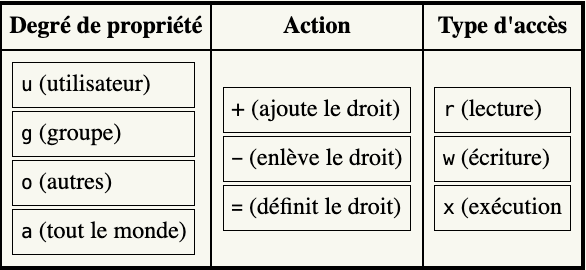
\includegraphics[scale=0.4]{chmod.png}
    \caption{chmod en notation symbolique}
     \end{center}
\end{figure}    

\emph{catégorie + opérations + liste\_droits} peuvent être par exemple :

\begin{itemize}
\tightlist
\item
  \texttt{u+r} pour rajouter au propriétaire le droit en lecture,
\item
  \texttt{g-w} pour retirer aux membres du groupe le droit en écriture,
\item
  \texttt{o+x} pour donner aux autres utilisateurs le droit en
  exécution,
\item
  ou une combinaison de ces possibilités (ex: \texttt{u-wx},
  \texttt{ug-w}, \texttt{ug-wx}).
\end{itemize}

\subsubsection{Protéger complètement un fichier } 

Ici, vous interdisez à tout autre que vous l'accès à votre script \texttt{monProgramme.py} (c'est ce qu'on appelle couramment le ``mode parano'', Figure 7). Vous retirez les droits de lecture au groupe (g) et aux autres (o) 

La commande utilisée est : \texttt{chmod} \emph{og-r} \underline{fichier(s)}

\begin{figure}[h!]
    \begin{center}
    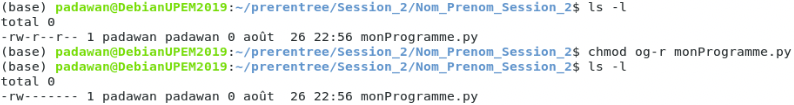
\includegraphics[scale=0.6]{fichier_Enlever_Droit.png}
    \caption{``mode parano''}
     \end{center}
\end{figure}   

\subsubsection{Rétablir des droits normaux pour un fichier } 

\begin{figure}[h!]
    \begin{center}
    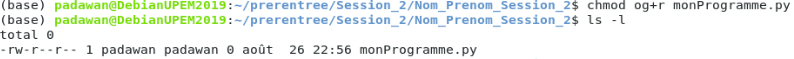
\includegraphics[scale=0.6]{fichier_Retablir_Droit.png}
    \caption{Rétablir les droits normaux du script \texttt{monProgramme.py} }
     \end{center}
\end{figure}   

\subsubsection{Protéger un répertoire} 

Comme pour un fichier on utilise aussi la commande \texttt{chmod}

\begin{figure}[h!]
    \begin{center}
    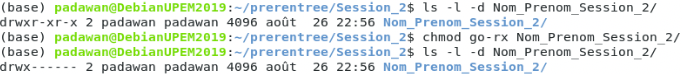
\includegraphics[scale=0.6]{rep_Enlever_Droit.png}
    \caption{``mode parano''}
     \end{center}
\end{figure}   

\subsubsection{Rétablir des droits normaux pour un répertoire} 

\begin{figure}[h!]
    \begin{center}
    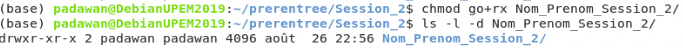
\includegraphics[scale=0.6]{rep_Retablir_Droit.png}
    \caption{Rétablir les droits normaux d'un répertoire}
     \end{center}
\end{figure}   

\hypertarget{Entraînez-vous}{
\subsection{Entraînez-vous}\label{Entraînez-vous}}

Dans cette partie deux exercices pour vous entraîner sur la gestion des droits :

\begin{itemize}
\item
un exercice sur la gestion des droits pour les fichiers
\item
un exercice sur la gestion des droits pour les répertoires
\end{itemize}

\begin{exercice}[Exécuter un fichier.]

\begin{enumerate}
\def\labelenumi{\arabic{enumi}.}
\item
  Créez un répertoire \texttt{Essai} (si vous n'en possédez pas déjà
  un), et un fichier \texttt{mon\_ls} dans ce répertoire, et écrivez-y
  quelques mots de votre choix.
\item
  Notez à l'aide de \texttt{ls\ -l} les permissions actuelles du
  répertoire \texttt{Essai} et du fichier \texttt{mon\_ls}.
\item
  En utilisant la commande \texttt{chmod}, retirez-vous le droit en
  lecture et en écriture sur le fichier \texttt{mon\_ls}. Vérifiez
  l'effet obtenu en essayant d'afficher le contenu du fichier sur la
  fenêtre du terminal avec la commande \texttt{cat}, puis de remplacer
  ce contenu par une phrase différente.
\item
  Un fichier exécutable est simplement un fichier dont vous possédez le
  droit en exécution. Rétablissez le droit en écriture puis remplacez le
  contenu du fichier \texttt{mon\_ls} par le texte
  \texttt{"echo\ Contenu\ du\ dossier;\ ls"}. Ajoutez-vous le droit en
  exécution, et exécutez le fichier \texttt{mon\_ls} en tapant
  \texttt{./mon\_ls} dans le terminal (depuis le répertoire qui le
  contient). Quel est le problème ?
\item
  Rétablissez enfin le droit en lecture et tentez à nouveau d'exécuter
  le fichier. Que se passe-t-il?
\end{enumerate}

\end{exercice}

Si le sens de chaque droit pour un fichier ordinaire est assez clair, il
est parfois moins intuitif pour un répertoire, comme vous le verrez dans
l'exercice suivant.

\begin{exercice}[Un test.]

\begin{enumerate}
\def\labelenumi{\arabic{enumi}.}
\item
  Placez-vous dans le répertoire \texttt{Essai}, et retirez-vous le
  droit en lecture pour ce répertoire. Listez le contenu du répertoire
  avec \texttt{ls}, puis exécutez ou affichez le contenu du fichier
  \texttt{mon\_ls}. Qu'en déduisez-vous ? Rétablissez le droit en
  lecture sur \texttt{mon\_ls} et sur \texttt{Essai}.
\item
  Créez dans \texttt{Essai} un fichier \texttt{nouveau} ainsi qu'un
  répertoire \texttt{Test}. Retirez au fichier \texttt{nouveau}
  \textbf{et} au répertoire \texttt{Essai} le droit en écriture. Tentez
  de modifier le fichier \texttt{nouveau}, de le déplacer, de le
  supprimer. Rétablissez ensuite le droit en écriture au répertoire
  \texttt{Essai}. Tentez de modifier le fichier \texttt{nouveau}, puis
  de le déplacer ou de le supprimer. Que constatez-vous ?
\item
  Positionnez-vous dans votre répertoire personnel, puis retirez le
  droit en exécution du répertoire \texttt{Essai}. Tentez de créer,
  supprimer, ou modifier un fichier dans le répertoire \texttt{Essai},
  de vous y déplacer, d'en faire la liste, etc. Qu'en déduisez-vous
  quant au sens du droit en exécution pour les répertoires ?
\end{enumerate}

\end{exercice}

\section {Bien suivre les cours et se former à Python}

Vous allez bientôt commencer votre formation en L1 ainsi que vos cours en algorithmique et programmation avec le langage Python. Ce chapitre est dédié à la présentation des outils et applications qui vous permettront de bien démarrer.

\subsection{Thonny : éditeur Python pour les cours d'AP1 (APP1 et autre ...)}

Quand on découvre un langage de programmation et surtout la logique algorithmique, il faut utiliser des outils simples, facile d'accès et de compréhension.

À la vérité quand on débute en Python, un simple éditeur de texte est très suffisant, comme vous avez pu le voir à l'exercice 9. 

Cependant, plus on progresse dans les subtilités du langage et plus on a envie d'aller un peu plus ``vite'' et de bénéficier d'un éditeur de texte plus convivial, plus riche de fonctionnalités d'assistance comme par exemple la complétion de code ou la coloration syntaxique du langage (Il s'agit d'un formatage automatique du texte avec une couleur et une fonte spécifique en fonction de son type : variable, fonction, ...). \\
Bref on parle ici d'IDE (Integrated Development Environment), soit en fran\c cais; Environnement Intégré de Développement.

Sur internet, dans votre entourage et auprès de vos collègues des années précédentes vous trouverez et entendrez parler d'une multitude d'IDEs tous plus pointus et complets les uns les autres. Néanmoins, plus pointu et plus complet veut dire aussi plus complexe voir beaucoup plus complexe et il y a de fortes chances pas très utile pour le niveau d'une L1 (qu'on soit en MIASHS, AP1 ou en APP1) ! \\
Des IDEs comme PyCharm, Visual Studio Code (VS Code) ou Spyder peuvent être très séduisants et ont pignon sur internet (\c ca veut dire qu'internet ne jurent que par eux). Ces IDEs font littéralement le café ... à la condition de savoir s'en servir ... à la condition d'en avoir réellement besoin aussi. \\
Pour résumer, un IDE aussi fantastique soit-il ne codera jamais pour vous ! Il s'agit avant tout d'un assistant éditeur ``intelligent'' pour faciliter la vie des développeurs. 

Soyons clair, personne ne vous empêchera de choisir l'IDE que vous voudrez tant que vous faites, avec ce dernier, ce qui est demandé pendant vos cours.

Pour vous faciliter la vie, l'équipe enseignante d'AP1 vous propose l'IDE Thonny : \url{https://thonny.org/}. Thonny est un IDE très simple et très adapté à vos premiers pas sur Python. 

Dans cette section, l'objectif n'est pas de vous former à Thonny mais de vous donner les moyens de le faire et éventuellement de l'installer sur vos machines perso. Il y a d'ailleurs un tuto sympa en fran\c cais que vous pourriez suivre pour vous former : \url{https://www.codeflow.site/fr/article/python-thonny}.

\subsection{Python Tutor}

Dans la série des outils qui vous aideront à survivre à vos cours de L1 et potentiellement même après (avec d'autres langages), 
Python Tutor est un must (\url{https://pythontutor.com/}) ! 

Cet outil permet de visualiser en live le déroulement d'un programme ligne par ligne en présentant les variables dans un graphique très intuitif. Il a aussi l'avantage de ne pas nécessiter d'installation. 

Python Tutor est un outil pédagogique qui est très largement utilisé par les enseignants. Savoir l'utiliser serait un plus. 

À ce sujet regardez la vidéo sous Elearning : \emph{``PythonTutor.mov''}.

\textbf{ATTENTION : Il ne s'agit pas d'un IDE, vous ne pourrez pas programmer avec ! Vous ne pourrez pas sauvegarder votre code naturellement non plus ... puisque ce n'est pas un IDE.}

\subsection{La plateforme PLaTon}

PLaTon pour \textbf{PLatform for Learning and Teaching online} est un exerciseur pédagogique multi-matières open-source crée à l'Institut Gaspard Monge (soit l'UGE). 

C'est une manière de s'entrainer via des exercices qui vous permettront de conforter et de développer vos connaissances en Python (parfois même de s'entraîner avant les examens ...). PLaTon peut être vu un peu comme WIMS, les exercices sont à faire en autonomie et les corrections sont automatiques (exercices auto-corrigés).

Les exercices PLaTon ne sont pas notés et pas du tout obligatoires, c'est cependant un bon moyen de s'entraîner et de pratiquer, voire d'aller plus loin. 

L'accès à PLaTon (pour les exos Python) se fait en étant connecté à Elearning via le lien présent sous Elearning de la ``Pré Rentrée L1 2022/23'' (et pas autrement !!!). C'est une question de droit d'accès. 

Cliquez sur le lien ``Python\_L1\_Entrainement-22\_23'', une fois connecté vous verrez apparaître la fenêtre suivante : 

\begin{figure}[h!]
    \begin{center}
    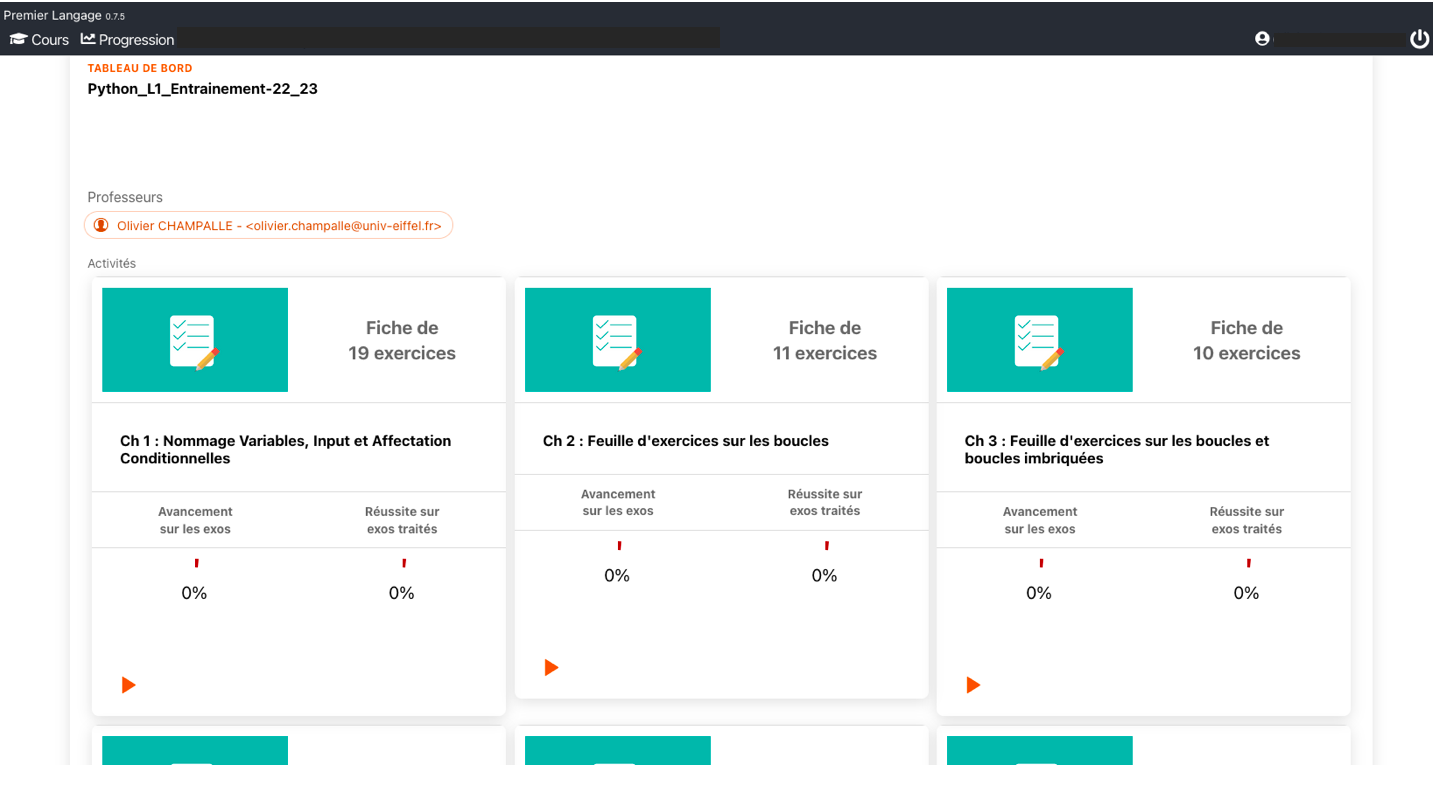
\includegraphics[scale=0.3]{PLaTon1.png}
    \caption{Page des exercices de Python en libre service pour les L1}
     \end{center}
\end{figure}   

La fenêtre de la figure 11 met à disposition l'ensemble des chapitres d'exercices Python actuellement disponibles. 

Pour démarrer une série d'exercices il faut cliquer sur la flèche orange d'un chapitre afin d' accéder à la page d'accueil du chapitre en question (figure 12). 

Un clique sur le bouton vert ``Commencer'' (figure 12) lancera le premier exercice de la série. Vous pouvez même directement cliquer sur n'importe quel exercice dans l'ordre que vous désirez.

La vidéo ``Presentation\_PLaTon.mov'' sous Elearning vous présente le fonctionnement sur deux exercices.

\begin{figure}[h!]
    \begin{center}
    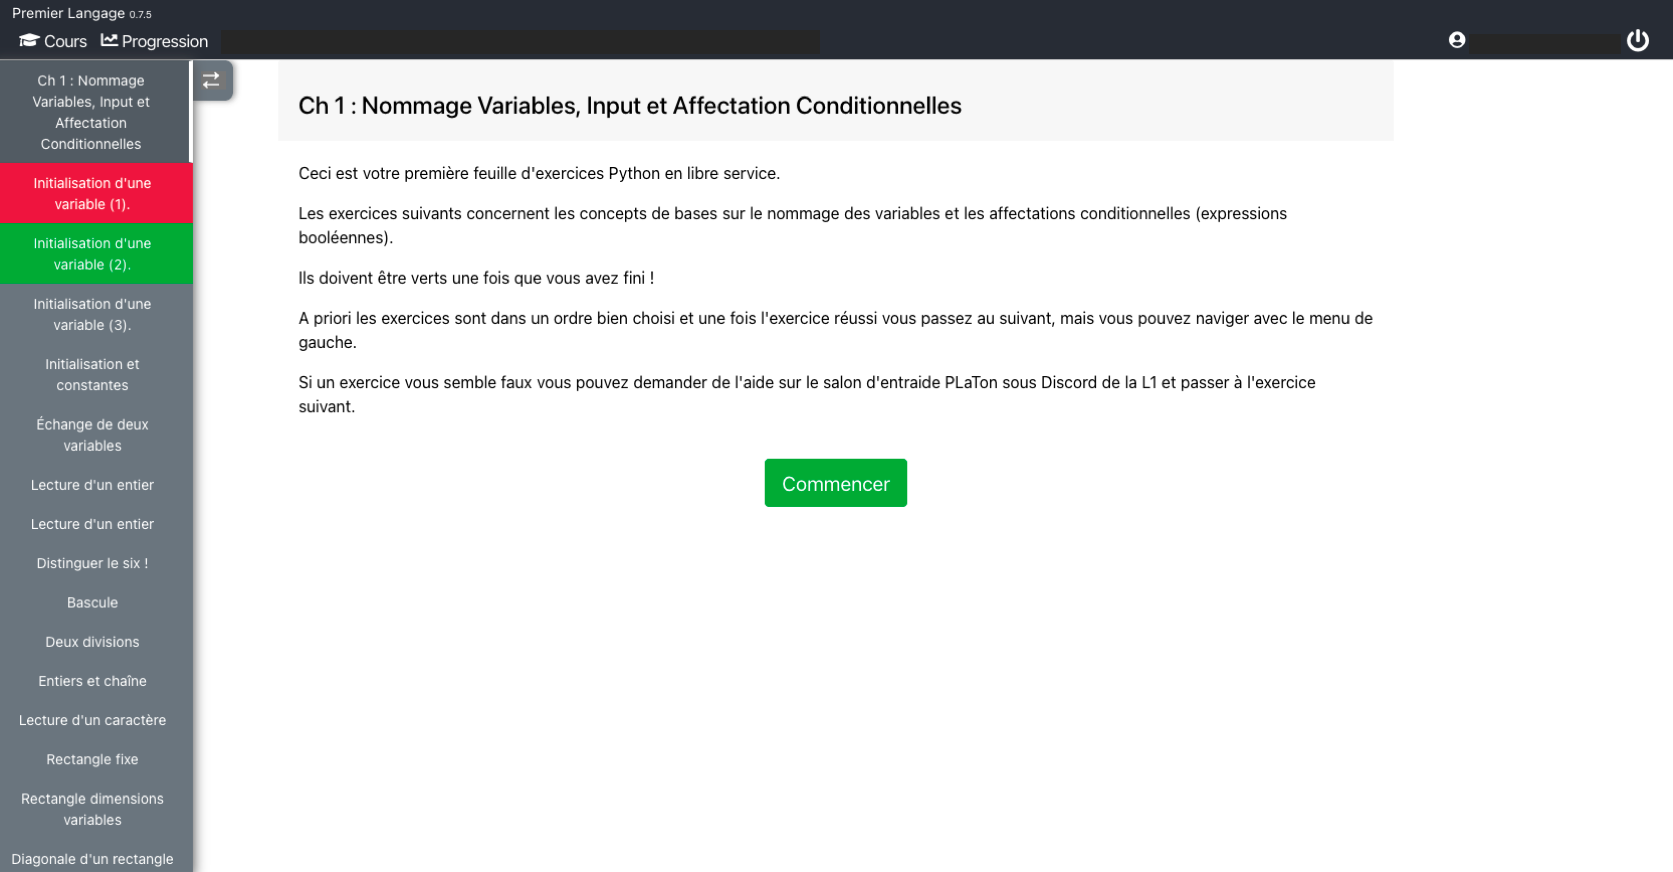
\includegraphics[scale=0.25]{PLaTon2.png}
    \caption{Ch1 : Nommage Variables, Input et Affectation Conditionnelles}
     \end{center}
\end{figure}   

Voilà c'est la fin de la Session\_2 ! 

A présent vous êtes formés et préparés pour entrer de plein pied dans votre formation ! 

Nous vous souhaitons une pleine et complète réussite.

\end{document}